\renewcommand{\algorithmicrequire}{\textbf{Input:}}
\renewcommand{\algorithmicensure}{\textbf{Output:}} 

\section{paper2's title}

\subsection{Motivation}

\begin{equation}
\begin{aligned} 
    \widehat{f} = & \operatorname{argmin}_{f} - f^{T} s + \frac{1}{2} f^{T} K f \\ 
    &\text{s.t.}\sum_{i=1}^{n}f_{i}=1,\quad f_{i}\geq0
\end{aligned}
\label{equ:max_div}
\end{equation}

\begin{algorithm}
\caption{SMGS}
\label{alg:gs}
\begin{algorithmic}
    \REQUIRE ~~\\
    original uncertainty values $s$, similarity matrix $Q$, \\
    labeled set $L$, unlabeled set $U$
    \STATE \textbf{Initialization:} Set $s^1 = s$
    \FOR{$t = 1:B_q$}
        \STATE Choose $k^t = arg \max_{j\in U} q^T_j s^t$ from $U$
        \STATE Compute $f_{k^t}$ by $$ f_{k^t} = arg \min_{f_{k^t}} ||f_{k^t} q_{k^t} - s^t||^2.$$
        \STATE Update the uncertainty values for the next iteration.
        \STATE using $$s^{t+1} = max(s^t - f_{k^t}, 0).$$
        \STATE Move sample index $k^t$ from $U$ to $L$.
    \ENDFOR
    \ENSURE ~~ updated labeled set L
\end{algorithmic}
    \label{code:SMGS}
\end{algorithm}



\begin{figure}[ht!]
    \centering
    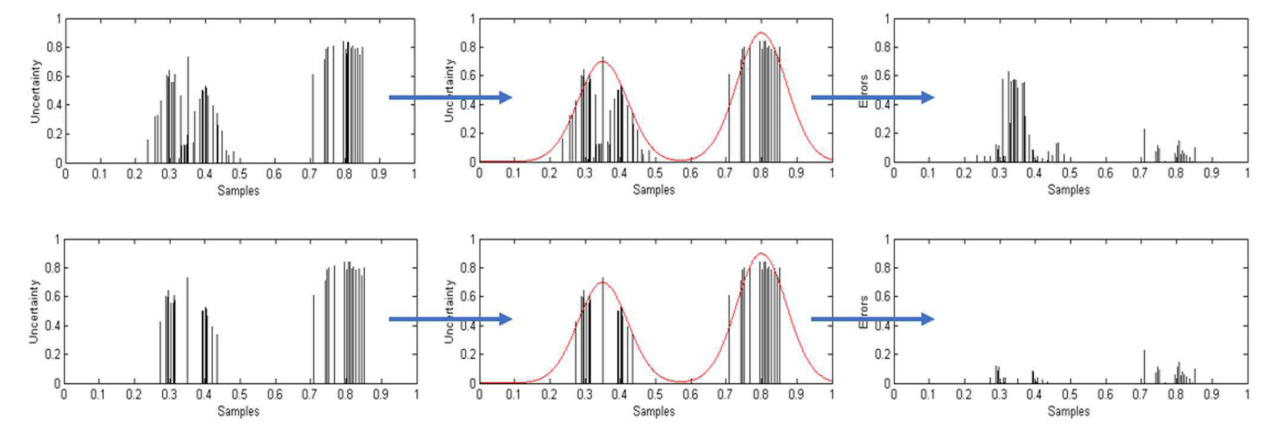
\includegraphics[width=10.4cm]{sparse_selective.png}
    \caption{The overview}
    \label{sparse_time}
\end{figure}

The Figure.\ref{sparse_time} shows the idea.


\begin{table}[t]
\caption{test table}
\label{test-case}
\begin{center}
\begin{threeparttable}
\begin{tabular}{lc}
% \hline \\[-1em]
\toprule
\multirow{2}{*}{Method} & Test Accuracy (\%) \\
                        & again              \\
% \hline \\[-1em]
\midrule
Supervised              & 55.44              \\
better model            & 59.71              \\
\midrule
best model              & \textbf{61.76}     \\ 
% \hline
\bottomrule
\end{tabular}
\end{threeparttable}
\end{center}
\vspace{-6mm}
\end{table}

\[
\begin{matrix}
d_{11} & d_{12} & d_{13} & \dots & d_{1n}\\
  & d_{22} & d_{23} & \dots & d_{2n}\\
  &  & d_{33}       &\dots & d_{3n}\\
  &  &              &\ddots & \vdots\\
  &  &              &       & d_{nn}
\end{matrix}
\]
